\title{14. Vztahy geometrických útvarů v rovině\\ - shodnost}
\author{Jonáš Lavička}
\date{2.5.2025}

\maketitle

\section{Vztahy geometrických útvarů v rovině\\ - shodnost}
     \subsection{Základní pojmy pro geometrická zobrazení}
        \begin{itemize}
            \item Geometrickým zobrazením $Z$ v rovině nazýváme zobrazení dané roviny na sebe, kterým každému  bodu $X$ je přiřazen právě jeden $X'$. Bod $X$ je vzor a bod $X'$ jeho obraz.\\
            Píšeme: $Z: X \rightarrow X'$ 
            \item Samodružný bod $X$ je bod pro který platí: $X = X'$
            \item Samodružný útvar $U$, je útvar pro který platí: $U = U'$\\
            Útvar $U$ se zobrazuje sám do sebe, je tvořen samodružnými body a body, které se zobrazují do jiných bodů útvaru - útvar je symetrický.
            \item Identita (identické zobrazení) je zobrazení, ve kterém je každý bod samodružný: $X=X'$
        \end{itemize}

    \subsection{Shodné zobrazení}
        Shodné zobrazení je v geometrii takové zobrazení, které záchovává vzdálenost.\\
        Každým dvěma bodům $X,Y$ přiřazuje body $X',Y'$ (obrazy) tak, že platí:\\
        \[\left| XY \right| = \left| X'Y' \right|\]
        Jsou li všechny odpovídající úsečky(páry bodů) dvou geometrických útvarů stejně dlouhé, jsou tyto útvary shodné.
        
    \subsection{Druhy shodnosti}
        V rovině existují následující druhy shodnosti:
        \subsubsection{Posunutí (translace) $T(\vec s)$}
            Všechny body roviny jsou posunuty stejným směrem o stejnou vzdálenost - směr a vzdálenost jsou dány \textbf{vektorem posunutí $\vec s$}.\\
            Platí: $X'=X+\vec s$\\
            V tomto zobrazení samodružný bod neexistuje.\\
            Všechny přímky rovnoběžné s vektorem posunutí $\vec s$ jsou samodružné.

            \begin{figure}[H]
                \centering
                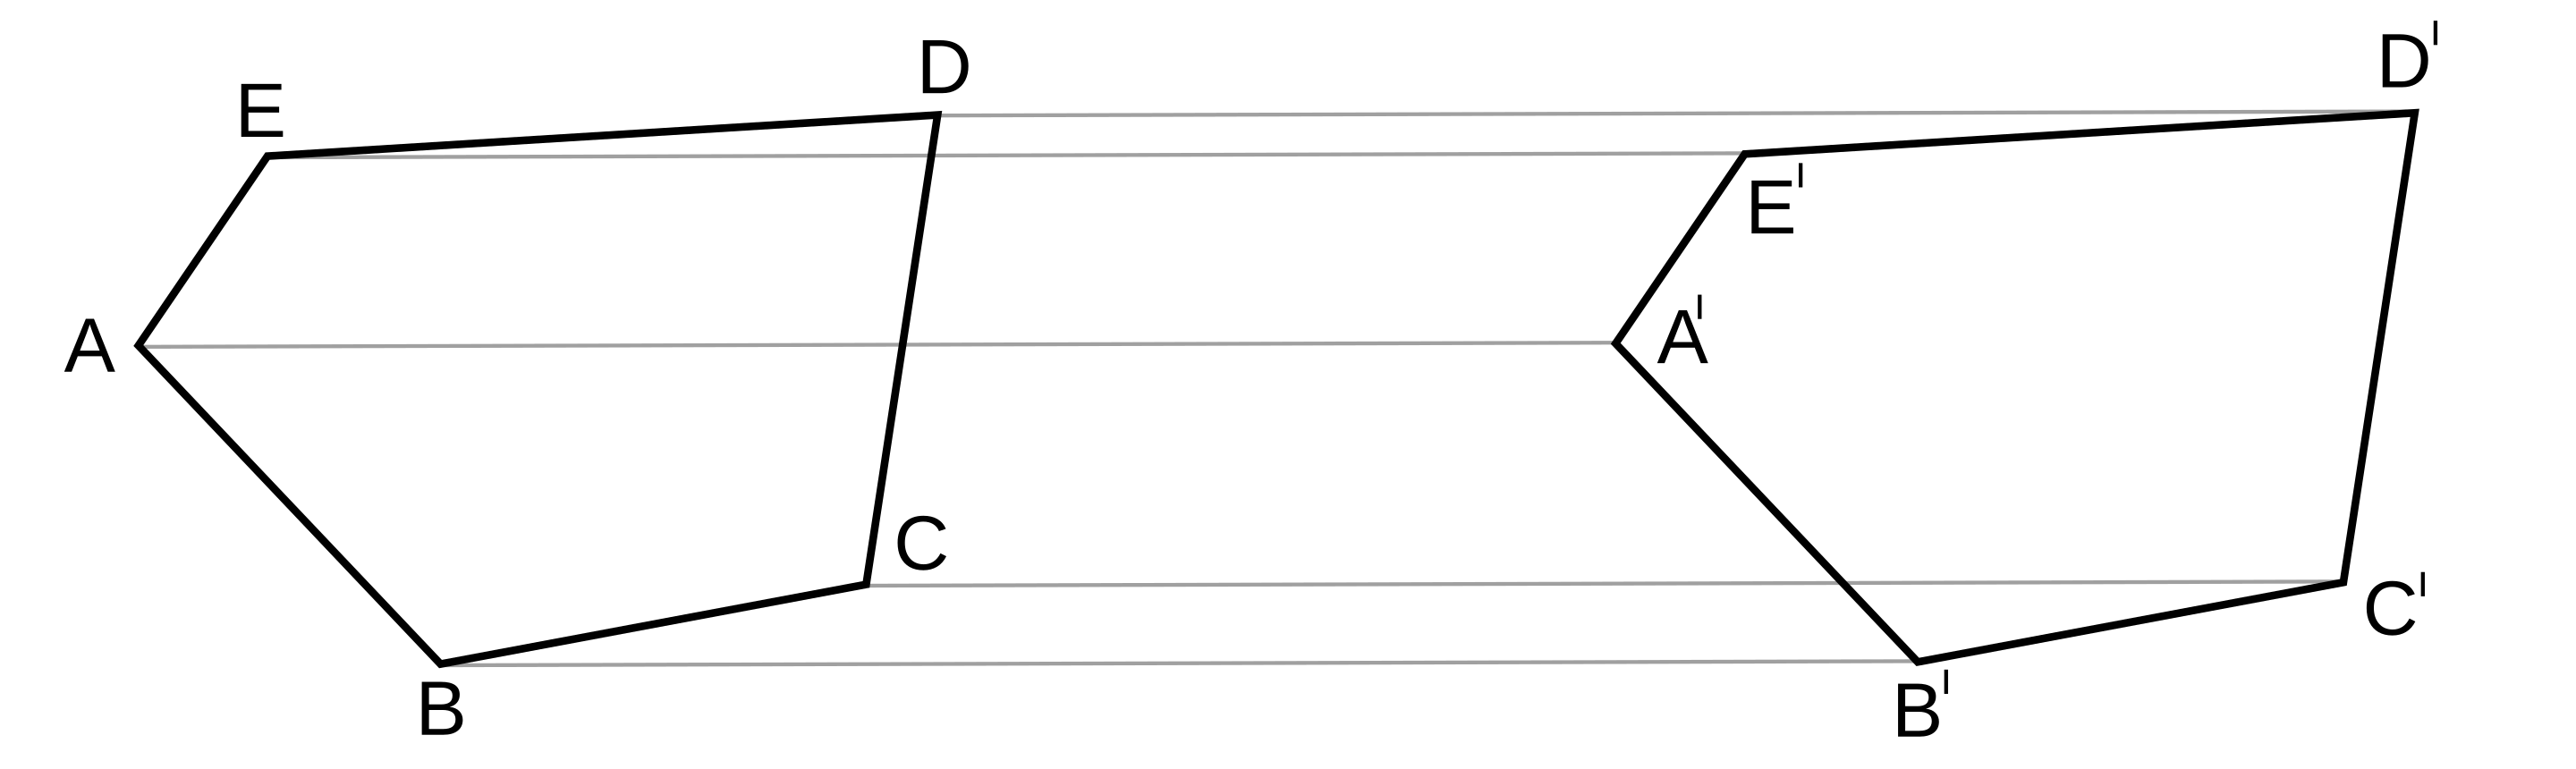
\includegraphics[width=0.5\linewidth]{img/19_posunuti.png}
                \caption{Posunutí pětiúhelníku} 
                \label{fig:enter-label}
            \end{figure}
            
        \subsubsection{Otočení (rotace) $O(S, \phi)$}
            Všechny body roviny jsou otočeny kolem středu otočení $S$ stejným směrem o úhel $\phi$.\\
            \begin{itemize}
                \item Bodu $S$ přiřazuje týž bod: $S'=S$ \\
                \item Každému bodu $X \neq S$ přiřazuje bod $X'$ tak, že $\left| XS \right| = \left| X'S \right|$ a orientovaný úhel $\measuredangle XSX'$ má velikost $\phi$.\\
            \end{itemize}
            Střed $S$ je samodružný bod.\\
            Pro $\phi = 180^{\circ}+k \cdot 360^{\circ};k \in \mathbb{Z} $ (liché násobky $180^{\circ}$), se jedná o středovou souměrnost.\\
            Pro $\phi = k \cdot 360^{\circ};k \in \mathbb{Z} $ (násobky $360^{\circ}$), se jedná o identitu.

            \begin{figure}[H]
                \centering
                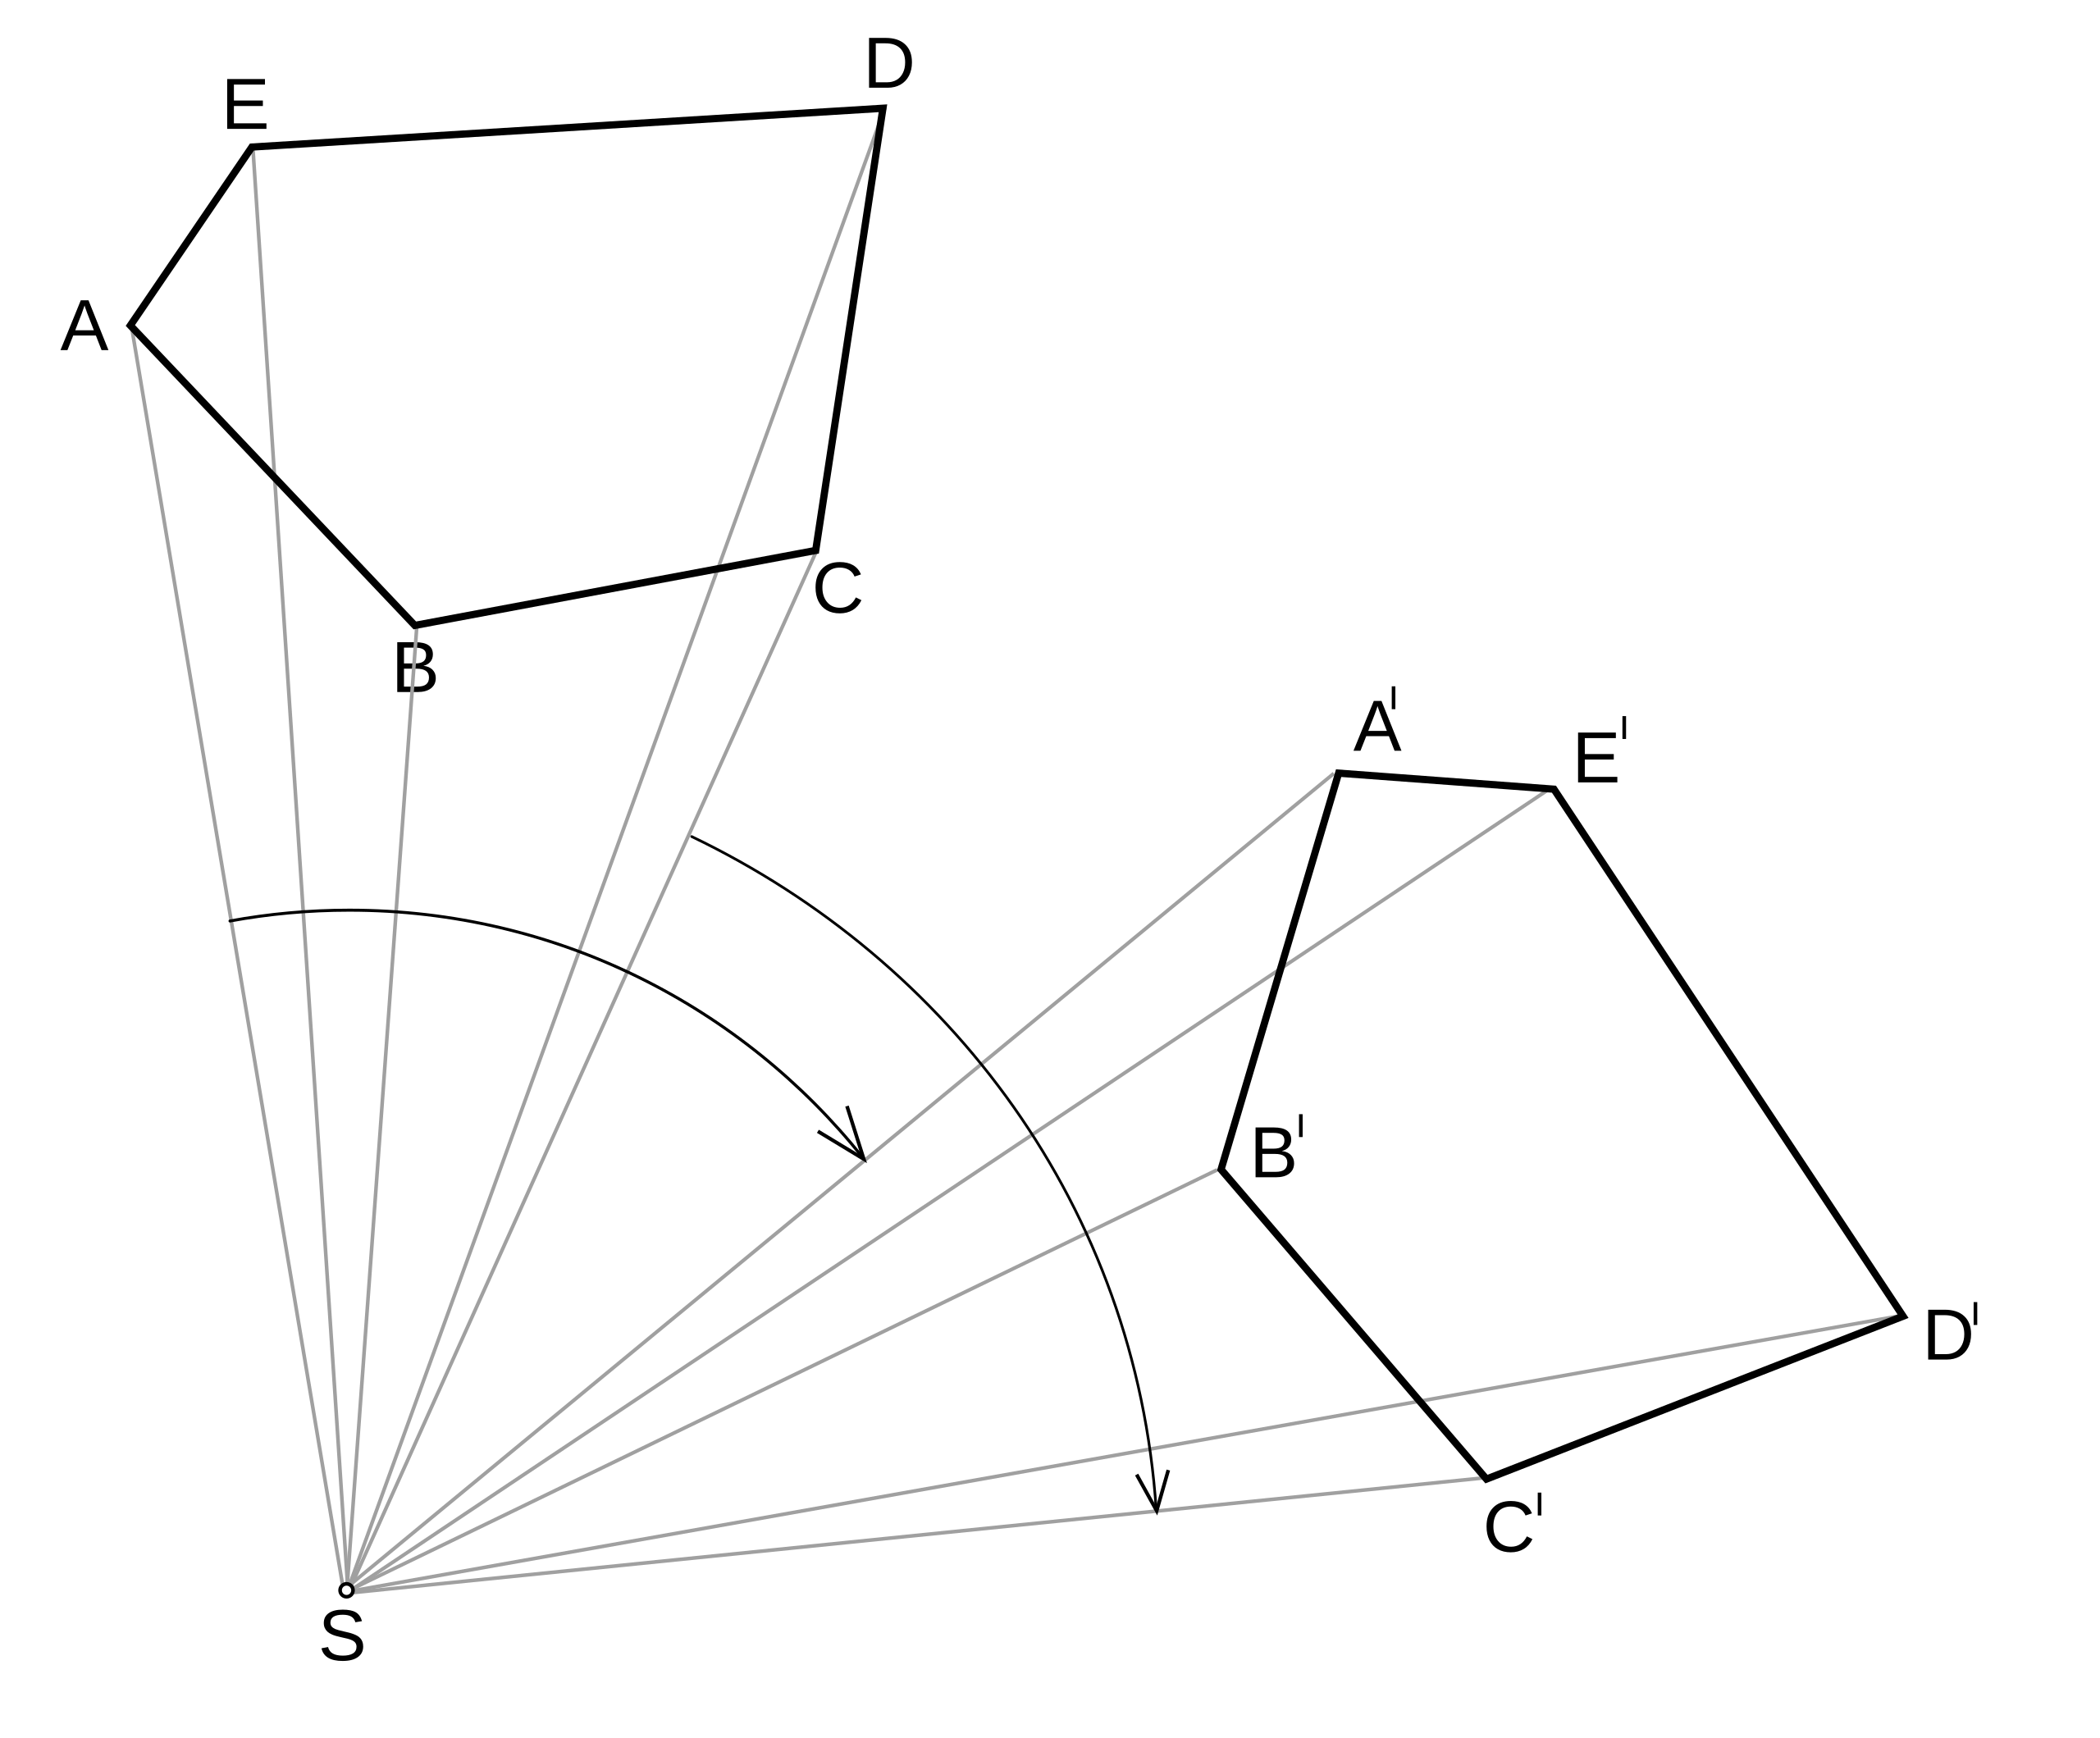
\includegraphics[width=0.5\linewidth]{img/19_otoceni.png}
                \caption{Otočení pětiúhelníku} 
                \label{fig:enter-label}
            \end{figure}
            
        \subsubsection{Středová souměrnost $S(S)$}
            Středová souměrnost je zvláštní případ otočení - otočení kolem středu o $180^{\circ}$.\\
            \begin{itemize}
                \item Středu souměrnosti $S$ přiřazuje týž bod: $S'=S$\\
                \item Bodu $X \neq S$ přiřazuje bod $X'$, který leží na polopřímce opačné k polopřímce $\mapsto SX$. Úsečka $XX'$ je bodem $S$ půlena.\\
            \end{itemize}
            Platí: $X' \in \; \mapsto XS \;\;\; \cap \;\;\; \left| XS \right| = \left| X'S \right| \;\;\; \cap \;\;\; X \neq X'$\\
            Střed $S$ je samodružný bod.

            \begin{figure}[H]
                \centering
                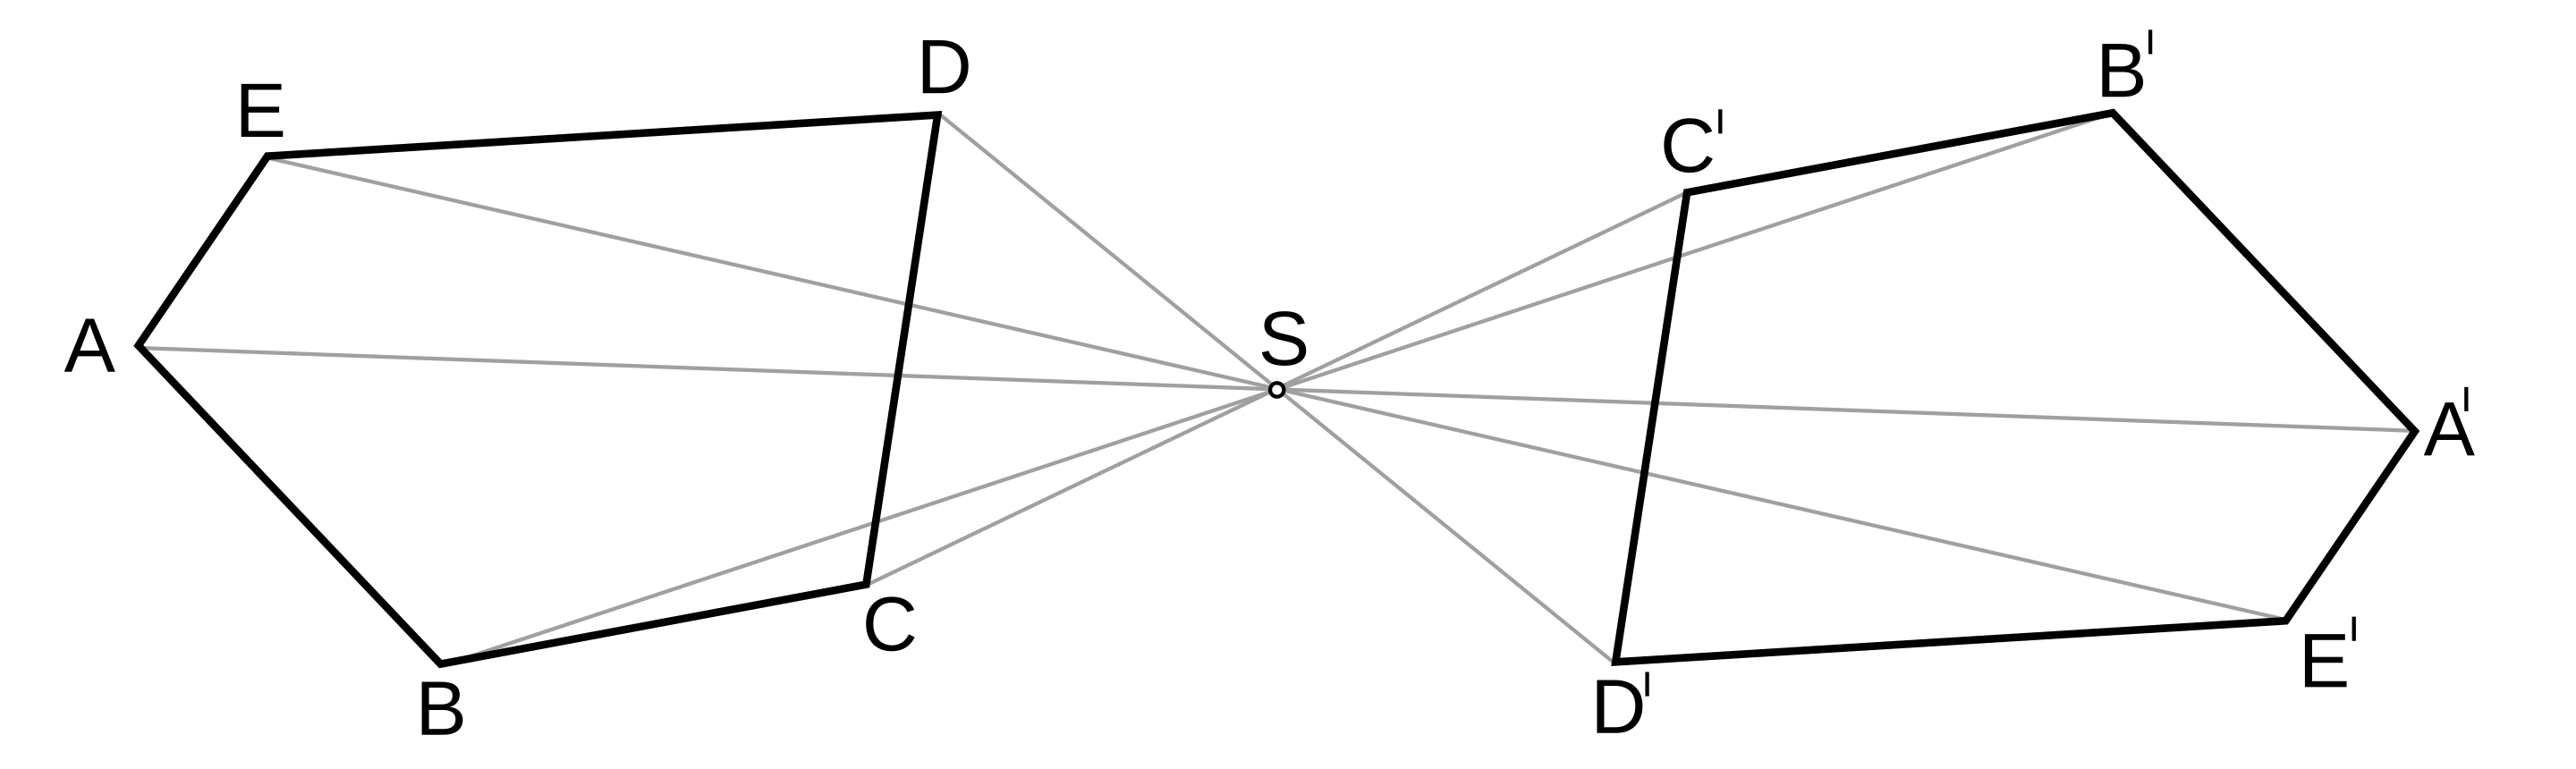
\includegraphics[width=0.5\linewidth]{img/19_stredova_soumernost.png}
                \caption{Zobrazení pětiúhelníku v středové souměrnosti} 
                \label{fig:enter-label}
            \end{figure}
            
        \subsubsection{Osová souměrnost(zrcadlení) $O(o)$}
            Osová souměrnost je shodné zobrazení, které je dané přímkou $o$ a zobrazovacím předpisem:\\
            \begin{itemize}
                \item Každému bodu $X \in o$ přiřazuje týž bod: $X'=X$
                \item Každému bodu $X \notin o$ přiřazuje bod $X'$, který leží na kolmici vedené bodem $X$ k ose $o$ tak, že úsečka $\leftrightarrow XX'$ je osou o půlena.
            \end{itemize}
            Platí: $X' \in \; \mapsto XS \;\;\; \cap \;\;\; \left| Xo \right| = \left| X'o \right| \;\;\; \cap \;\;\; X \neq X'$\\
            Všechny body osy $o$ jsou samodružné body - osa $o$ je samodružná přímka.\\
            Všechny přímky kolmé na osu $o$ jsou samodružné.

            \begin{figure}[H]
                \centering
                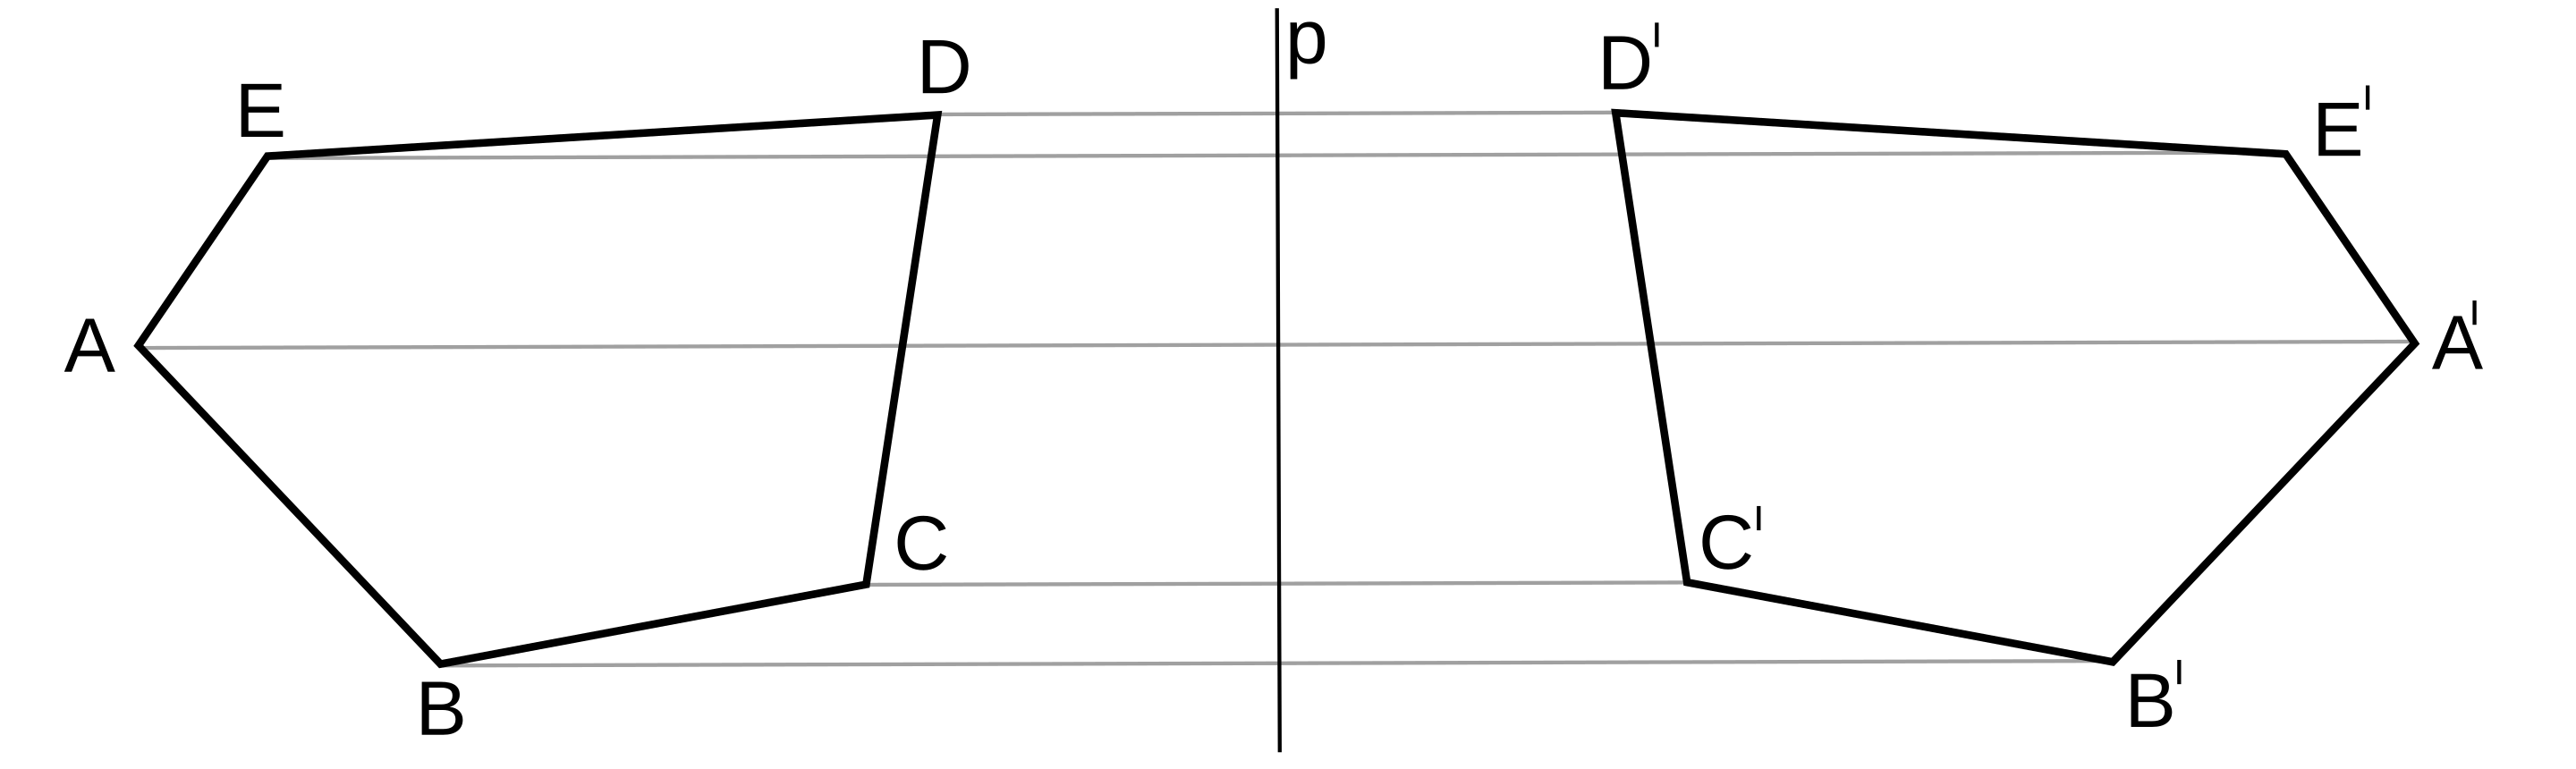
\includegraphics[width=0.5\linewidth]{img/19_osova_soumernost.png}
                \caption{Zobrazení pětiúhelníku v osové souměrnosti} 
                \label{fig:enter-label}
            \end{figure}
            
        \subsubsection{Totožnost (identita) $I()$}
            Zobrazení, které každý bod zobrazuje na sebe sama. Lze ji považovat za posunutí o úsečku nulové délky nebo za otočení o nulový úhel.\\
            Každý bod je samodružný.

            \begin{figure}[H]
                \centering
                
\includegraphics[width=0.5\linewidth]{img/19_identita.png}
                \caption{Geometrická identita} 
                \label{fig:enter-label}
            \end{figure}
            
    \subsection{Skládání shodných zobrazení}
        Shodné zobrazení shodného zobrazení je jen dalsí shodné zobrazení.
        \begin{itemize}
            \item Složením dvou posunutí je opět posunutí.
            \item Složením dvou středových souměrností je posunutí.
            \item Složením dvou otočení se stejným středem je opět otočení se stejným středem.
            \item Složením dvou osových souměrností se stejnou osou je identita.
            \item Složením dvou osových souměrností s různými rovnoběžnými osami je posunutí.
            \item Složením dvou osových souměrností s různoběžnými osami je otočení kolem průsečíku os, úhel $\phi$ je dvojnásobek úhlu, který osy svírají.
        \end{itemize}

    \subsection{Přímá a nepřímá shodnost}
        Vrcholy vzorového trojúhelníku jsou pojmenovány proti směru hodinových ručiček.\\
        Po posunutí, otočení, středové souměrnosti si trojúhelník \textbf{zachová orientaci}. Trojúhleník je \textbf{přímo shodný}.\\
        Naopak po osové souměrnosti se pořadí vrcholů otočí. Osová souměrnost \textbf{mění orientaci}. Trojúhleník je \textbf{nepřímo shodný}.\\
        Shodnost zachovávající orientaci se nazývá přímá neboli přemístění. Shodnost měnící orientaci se nazývá nepřímá.\\
        \begin{itemize}
            \item Složením přímých shodností je přímá shodnost.
            \item Složením sudého počtu nepřímých shodností je přímá shodnost.
            \item Složením lichého počtu nepřímých shodností je nepřímá shodnost.
        \end{itemize}